\chapter{Combinatorics}
\label{cha:combinatorics}

Combinatorics, namely \textit{Combinatorial Mathematics}, mainly studies
\textit{permutation} and \textit{combination} of a \textit{set} or \textit{multiset}.

组合数学里经常要用到\textbf{映射}的概念,在后文的描述里,会多次出
现\textbf{对应}这样的字眼,表示两个集合间元素的映射。通常为了方便
分析,把元素、对象的不同用\textbf{编号}、\textbf{颜色}等标签来表示。

\section{Set and Multiset}
\label{sec:set-multiset}

组合数学问题总要对某个集合的元素进行操作,虽然我们通常不需要特别说明。
如~10~个人进行全排列,那么对应的集合由这~10~个人组成。

普通集合如:
\[ S = \{\, a_1,\, a_2,\, a_3,\, \dots,\, a_n\, \},\; i \in
  \mathbb{Z}: i \in [1, n] \]
表示有~$n$~种\textbf{不同}元素,并且每种元素只有一个,
称~$S$~为\textbf{单重集(合)}。

更一般的,\textbf{多重集(合)}:
\[ M = \{\; n_1 \cdot a_1,\; n_2 \cdot a_2,\; \dots,\; n_k \cdot a_k\; \} \]
突出元素\textbf{种类},即~$a_i$~表示第~$i$~种元素,而~$n_i$~则表
示第~$i$~种元素的个数。通常元素总个数用~$n$~表示:
\[ n = n_1\, +\, n_2\, +\, \dots\, +\, n_k \]
不难发现,单重集是多重集的特例,
此时
\[ k = n,\, n_i = 1,\, i \in \mathbb{Z}: i \in [1,k] \]
如果多重集里每种元素有无限个,则记为:
\[ M = \{\; \infty \cdot a_i,\; \infty \cdot a_2,\; \dots,\; \infty \cdot a_k\; \} \]
普通集合和普通排列组合对应,多重集合和多重排列组合对应,
这也是在正式介绍排列组合前先说下集合的定义。

排列组合里,集合元素通常都具体化为\textbf{不同}颜色小球,组合表示从
集合里取小球出来,而排列表示进一步把取出的小球排队,或放
进\textbf{不同}的盒子里,此时盒子的编号代表队列从头至尾的位置号。

注意符号表示的不同。单重集里~$n$~既表示元素种类和个数。而多重集
用~$k$~表示元素种数,用~$n$~和~$n_i$~表示个数。注意符号表示的
习惯:
\[ a_i,\, n_i,\, k,\, n,\, S,\, M \]

\section{Counting Principles}
\label{sec:counting-principles}

\uline{加法原理}:设集合~$S$~可以划分成若干不相交的子集~$S_1,\, S_2,\,
\cdots,\, S_m$,~则:
\[ |S| = |S_1| + |S_2| + \cdots + |S_m| \]

\uline{乘法原理}:设集合~$S$~是序偶~$(a, b)$~的集合,其中~$a$~来自于集
合~$A$, $b$~来自于集合~$B$. $A$~中每个元素~$a$~都要与~$B$~中每个元
素~$b$~配对。则:
\[ |S| = |A| \times |B| \]

\uline{减法原理}:设集合~$A$~是全集~$U$~的子集,补集
\footnote{用~overline, bar, complement,~或~smallsetminus~命令表示。
  后者的好处是同时指明了全集和子集。}\;
$\overline{A} = U \smallsetminus A = \{\, x\, |\, x\, \in U,\; x
\notin A \,\}$,~则:
\[ |A| = |U| - |\bar{A}| \]

\uline{除法原理}:设~$S$~是有限集,被划分为~$k$~个两两不相交的部分,
每部分皆有~$m$~个元素,则:
\[ k = \frac{|S|}{m} \]

后面会发现,很多应用都以单重集的排列、组合为原子操作,再结合计数四
原则完成。

\section{Permutation of Sets}
\label{sec:permutation-sets}

定义:从~$n$~个元素的单重集合~$S$~中,取出~$r$~个元素按次序排成一列,
称为~$S$~的一个~$r$-排列,记为:
\[ P(n,r),\, P_n^r,\, A_n^r \]
注意,定义里用~$r$~表示所取元素个数。

当~$r = n$~时,~$S$~的~$n$-排列简称为~$S$~的排列或~$n$~个元素
的\uline{全排列}。

从~$n$~个元素中取~$r$~个元素的排列的典型例子是从~$n$~个\textbf{不
  同}颜色的球中,取出~$r$~个,放入~$r$~个\textbf{不同}的盒子里,每
盒~1~个,盒子编号就映射成队列位置。显然第~1~个盒子有~n~种球可选,
第~2~个盒子有~$n-1$~种球可选,……,第~$i$~个盒子有~$n - (i - 1)$~种
球可选,……,第~$r$~个盒子有~$n - (r - 1)$~个球可选。

可以得出
\[ A_n^r = n(n - 1)\cdots[n - (i - 1)]\cdots[n - (r - 1)],\quad r \leq n,\quad n,\, r \in \mathbb{Z}^+ \]

定义阶乘~factorial~:
\begin{align*}
  n! &= n\times(n - 1)\times(n - 2)\cdots2\times1 \\
  0! &= 1
\end{align*}

排列组合是没会有~0~的情况的,但为了数学定义和计算的完备性,要考
虑~0~等情况。其实负数的阶成也有定义,不过在组合数学里没意义,在此不
考虑。后面还会遇到类似形式的定义。那么:

\begin{align*}
  A_n^r &= \frac{n!}{(n - r)!}, \quad 0 \leq r \leq n \\
  A_n^0 &= 1 \\
  A_n^n &= n!
\end{align*}

排列还分为\textbf{直线排列}和\textbf{圆排列}。直线排列就是我们常说
的排列,圆排列是指把取出的元素排成一个圆形,

上面定义的是\textbf{直排列},\textbf{圆排列}定义为取出的元素排成一
个圆圈,等于是让直线排列的首尾相连接。从~$n$~个元素中取出~$r$~个构
成的圆~$r$-排列数为:
\[ A_n^r/r,\quad (1 \leq r \leq n) \]因为~1~个圆排列从任一位置断开
都是一个不同的直排列,也就是说~$r$~个直排列对应~1~个圆排列,所以要
在直排列基础上\uwave{除以}~$r$.~注意,是除不是乘。 特殊的,$n$~个元
素的全圆排列数为~$(n - 1)!$.

圆排列还有一种情况是,可以翻转圆排列,如~$n$~个不同颜色的珠子串成一
条项链。一条项链的一面是一个普通圆排列,但翻转这个项链,它的另一面
是一个新有圆排列,所以每个可翻转圆排列对应~$2$~个普通圆排列。因
此,\textbf{可翻转圆排列}数为 \[ \frac{A_n^r}{2 \cdot n} \]

\section{Combination of Sets}
\label{sec:combination-sets}

上节讨论了单重集的排列,这节讲单重集的组合。排列和组合的主要区别
是\textbf{不同}元素是否有\textbf{次序}。组合取出元素\textbf{堆}在一
起,而排列在组合的基础上对取出的元素堆进行排队或入盒。

一旦取出,便不再区分组合堆内球的不同。如果取出多个堆,堆间区别
是\uwave{球的个数:堆内无序,堆间也无序}。后面多次用到这个
原则。

从~$S$~中取~$r$~个元素而不进行排序,称为~$S$~的一个~$r$-组合,实际
就是生成一个~$S$~的~$r$~元素子集,可以看成是取出元素堆在一起,没有
顺序:\uwave{组合即组堆,也即生成子集}。

组合的对应彩色球问题是从~$n$~个色彩\textbf{不同}的小球中取出~$r$~个
(堆在一起),此时没有放入盒子的操作:只取不入。如果一定要有入盒操
作,那么所有的盒子相同,没有编号区分,此时入盒与否没有意
义。~$r$~-组合数记为

\[ C(n,r),\, C_n^r,\, \binom{n}{r} \]

很显然,一个~$r$~-组合可以生成~$r!$~个排列,所以:
\begin{align*}
  C_n^r &=  \frac{A_n^r}{r!} = \frac{n!}{(n - r)!\,r!}, \quad r,\,
          n \in \mathbb{Z}_0^{+}: r \in [0, n] \\
  C_n^r &= 0, \quad r > n \\
  C_n^0 &= 1 \\
  C_n^n &= 1 \\
  C_0^0 &= 1
\end{align*}

从上面方程中的特例可以看出,完备性定义对数学计算的意义。阶乘,排列
数,组合数的完备性定义主要考虑~$r > n$~和~$n,\, r = 0$~的情况。一般
地,我们只考虑~$0 \leq r \leq n$~的情况。对于~$r,\, n < 0$~的情况
不在排列组合的讨论范围。在其它计算领域即便碰到,也不难,只要严格按
照阶乘的定义计算即可。

由公式:
\[ A_n^r = C_n^r\, r!,\quad r,\, n \in \mathbb{Z}_0^{+}: r \in [0,
  n] \]
可以得出,除原始定义外,排列操作可看作先取组合,得到一堆元素,再对
此堆列队。可以说\textbf{排列操作暗含了组合子问题}。简而言之,1 个组
合对应~$r!$~个排列,排列数是组合数的~$r!$~倍。后面更复杂的分配分组
问题也遵循此规律。

\subsection{Combination Formulas}
\label{sec:combination-formulas}

组合数的计算非常重要,因为组合公式是一个很重要的数学工具,如多项式
的系数和组合数紧密相联。本小节着重讲组合数的几个公式。

组合数和排列数计算都化成阶乘的计算。不过,当参数很大时,计算阶乘不
是件容易的事。但从组合数的原始定义可知:取~$r$~个元素得到一个子集,
余下的就是~$n - r$~元素的补集,一一对应。也就是说,每取一个~$(n -
r)$-组合就得到一个~$r$~-组合:
\[ C_n^r = C_n^{n - r}, \quad r,\, n \in \mathbb{Z}_0^{+}: r \in [0,
  n] \]
当~$r$~很大时,$n - r$~就很小,便于计算。我们还可以想办法降级阶数,
让其变得更小:
\[ C_n^r = C_{n - 1}^r + C_{n - 1}^{r - 1} \]
由此公式可得出
\href{https://zh.wikipedia.org/zh-hans/\%E6\%9D\%A8\%E8\%BE\%89\%E4\%B8\%89\%E8\%A7\%92\%E5\%BD\%A2}{
  杨辉三角形},也称~$Pascal$~三角形。

有趣的是让~$r$~遍历~$0$~到~$n$~,可以看出所有的组合数之和就是集
合~$S$~的幂集的元素个数:
\[ \sum_{r = 0}^n\binom{n}{r} = 2^n \]
此公式可以用二项式证明:
\[ (x + y)^n = \sum_{r = 0}^nC_n^rx^ry^{n - r}
\]令~$x,\, y = 1$~即可。

更一般地,组合公式的证明\textbf{双重计数~double counting}~法:从
不同(一般 2 种)角度对集合计数。更多关于双重计数,看~
\href{https://brilliant.org/wiki/double-counting-definition/}{Double
  Counting}~和
~\href{https://www.youtube.com/watch?v=TdtFxXo2zpg}{Mod-03 Lec-17
  Double counting - Part (2) }.

如上面的组合数求和公式,左边表示利用加法原则,以了集元素个数~$r$~来
对~$S$~的幂集计数。要证明,我们以另外一个角度来计数:利用乘法
原则,针对一个元素是否加入子集来计数。~$\forall a_i,\, 1 \leq i \leq
n$~要么在某个子集里,要么不在,只有两种可能。对~$a_i$~遍历,~$a_1$~有
两种可能,~$a_2$~有两种可能,……,~$a_n$~有两种可能,所以~$S$~有~$2
\times 2 \times \cdots \times 2 = 2^n$~个子集。

\subsection{Application of Combination}
\label{sec:appl-comb}

现有~$n$~个管理员管理
某\href{https://math.stackexchange.com/q/581461}{保密装
  置}(\href{https://math.stackexchange.com/q/1316831}{Minimum
  number of locks and keys})。要求任何~$\leq r$~个管理员都打不开该
装置,至少需~$r + 1$~个。假设该装置有~$s$~把钥匙,给每个管理员分配
其中的~$t$~把。问题是已知~$n,\, r,\; r \leq
n$,~求~$s,\, t,\; t \leq s$.~并进一步给出该装置的钥匙分配方案。

设管理员集合为:
\[ M = \{\, m_1,\, m_2,\, \cdots,\, m_n\, \},\; r \leq n \]
钥匙集合为:
\[ K = \{\, k_1,\, k_2,\, \cdots,\, k_s\, \},\; t \leq s \]

先求钥匙数~$s$.~由描述知,管理员集合~$M$~的任一~$r$-组合(管理员子
集)都不能凑齐~$s$~把钥匙,可知任一~$r$-组合至少还缺 1 把钥匙。显然,
任两个~$r$-组合的钥匙不能完全相同,也即不能缺同一把钥匙,否则~$2r$~个
管理员还因缺一个把钥匙而打不开保密装置,而且这样的分配方案没有意
义。~$M$~的~$r$-组合数是~$C_n^r$.~ 所以:\[ s \geq C_n^r\]

从上分析可看出,~$M$~的所有~$r$~元素子集到~$K$~的一个单射:每个~$r$元
素子集的像是它所缺失的那把钥匙。但它不一定是满射,因为~$s \gneq
C_n^r$~时,额外的钥匙会被所有的~$r$-组合所覆盖,这样的钥匙没的原像。
其中等号成立的条件是每个~$r$-组合刚好缺一把钥匙,此时构成一个满射。

再求每个管理员分得的钥匙数~$t$.
$M$~的任一~$(r + 1)$元素子集都能打开装置,说明其中任一管理员可补齐
剩下~$r$~个管理员所缺的那把钥匙。一个管理员~$m_l$~所参与的~$(r +
1)$-组合有~$C_{n - 1}^r$~个,所以:\[ t \geq C_{n - 1}^r \]

在分析钥匙的分发方案之前,让们回顾下上面的杨辉三角形,本题已出现公
式里两个分项~$C_n^r$~和~$C_{n - 1}^r$,~只不过后者的意义稍变了。

$s$~取最小值~$C_n^r$~时,我们列出~$M$~的所有~$r$~元素子集到~$K$~的
满射:\[ f(M_i) = k_j\]
\[ \{\, M_i \mid M_i \text{ is a set of size } r,\; i = 1,\,
  \cdots,\, C_n^r\, \} \xrightarrow{ \text{缺失} } K \]
显然这样的映射有很多种,我们只需选其一,如下图所示:

\begin{center}
  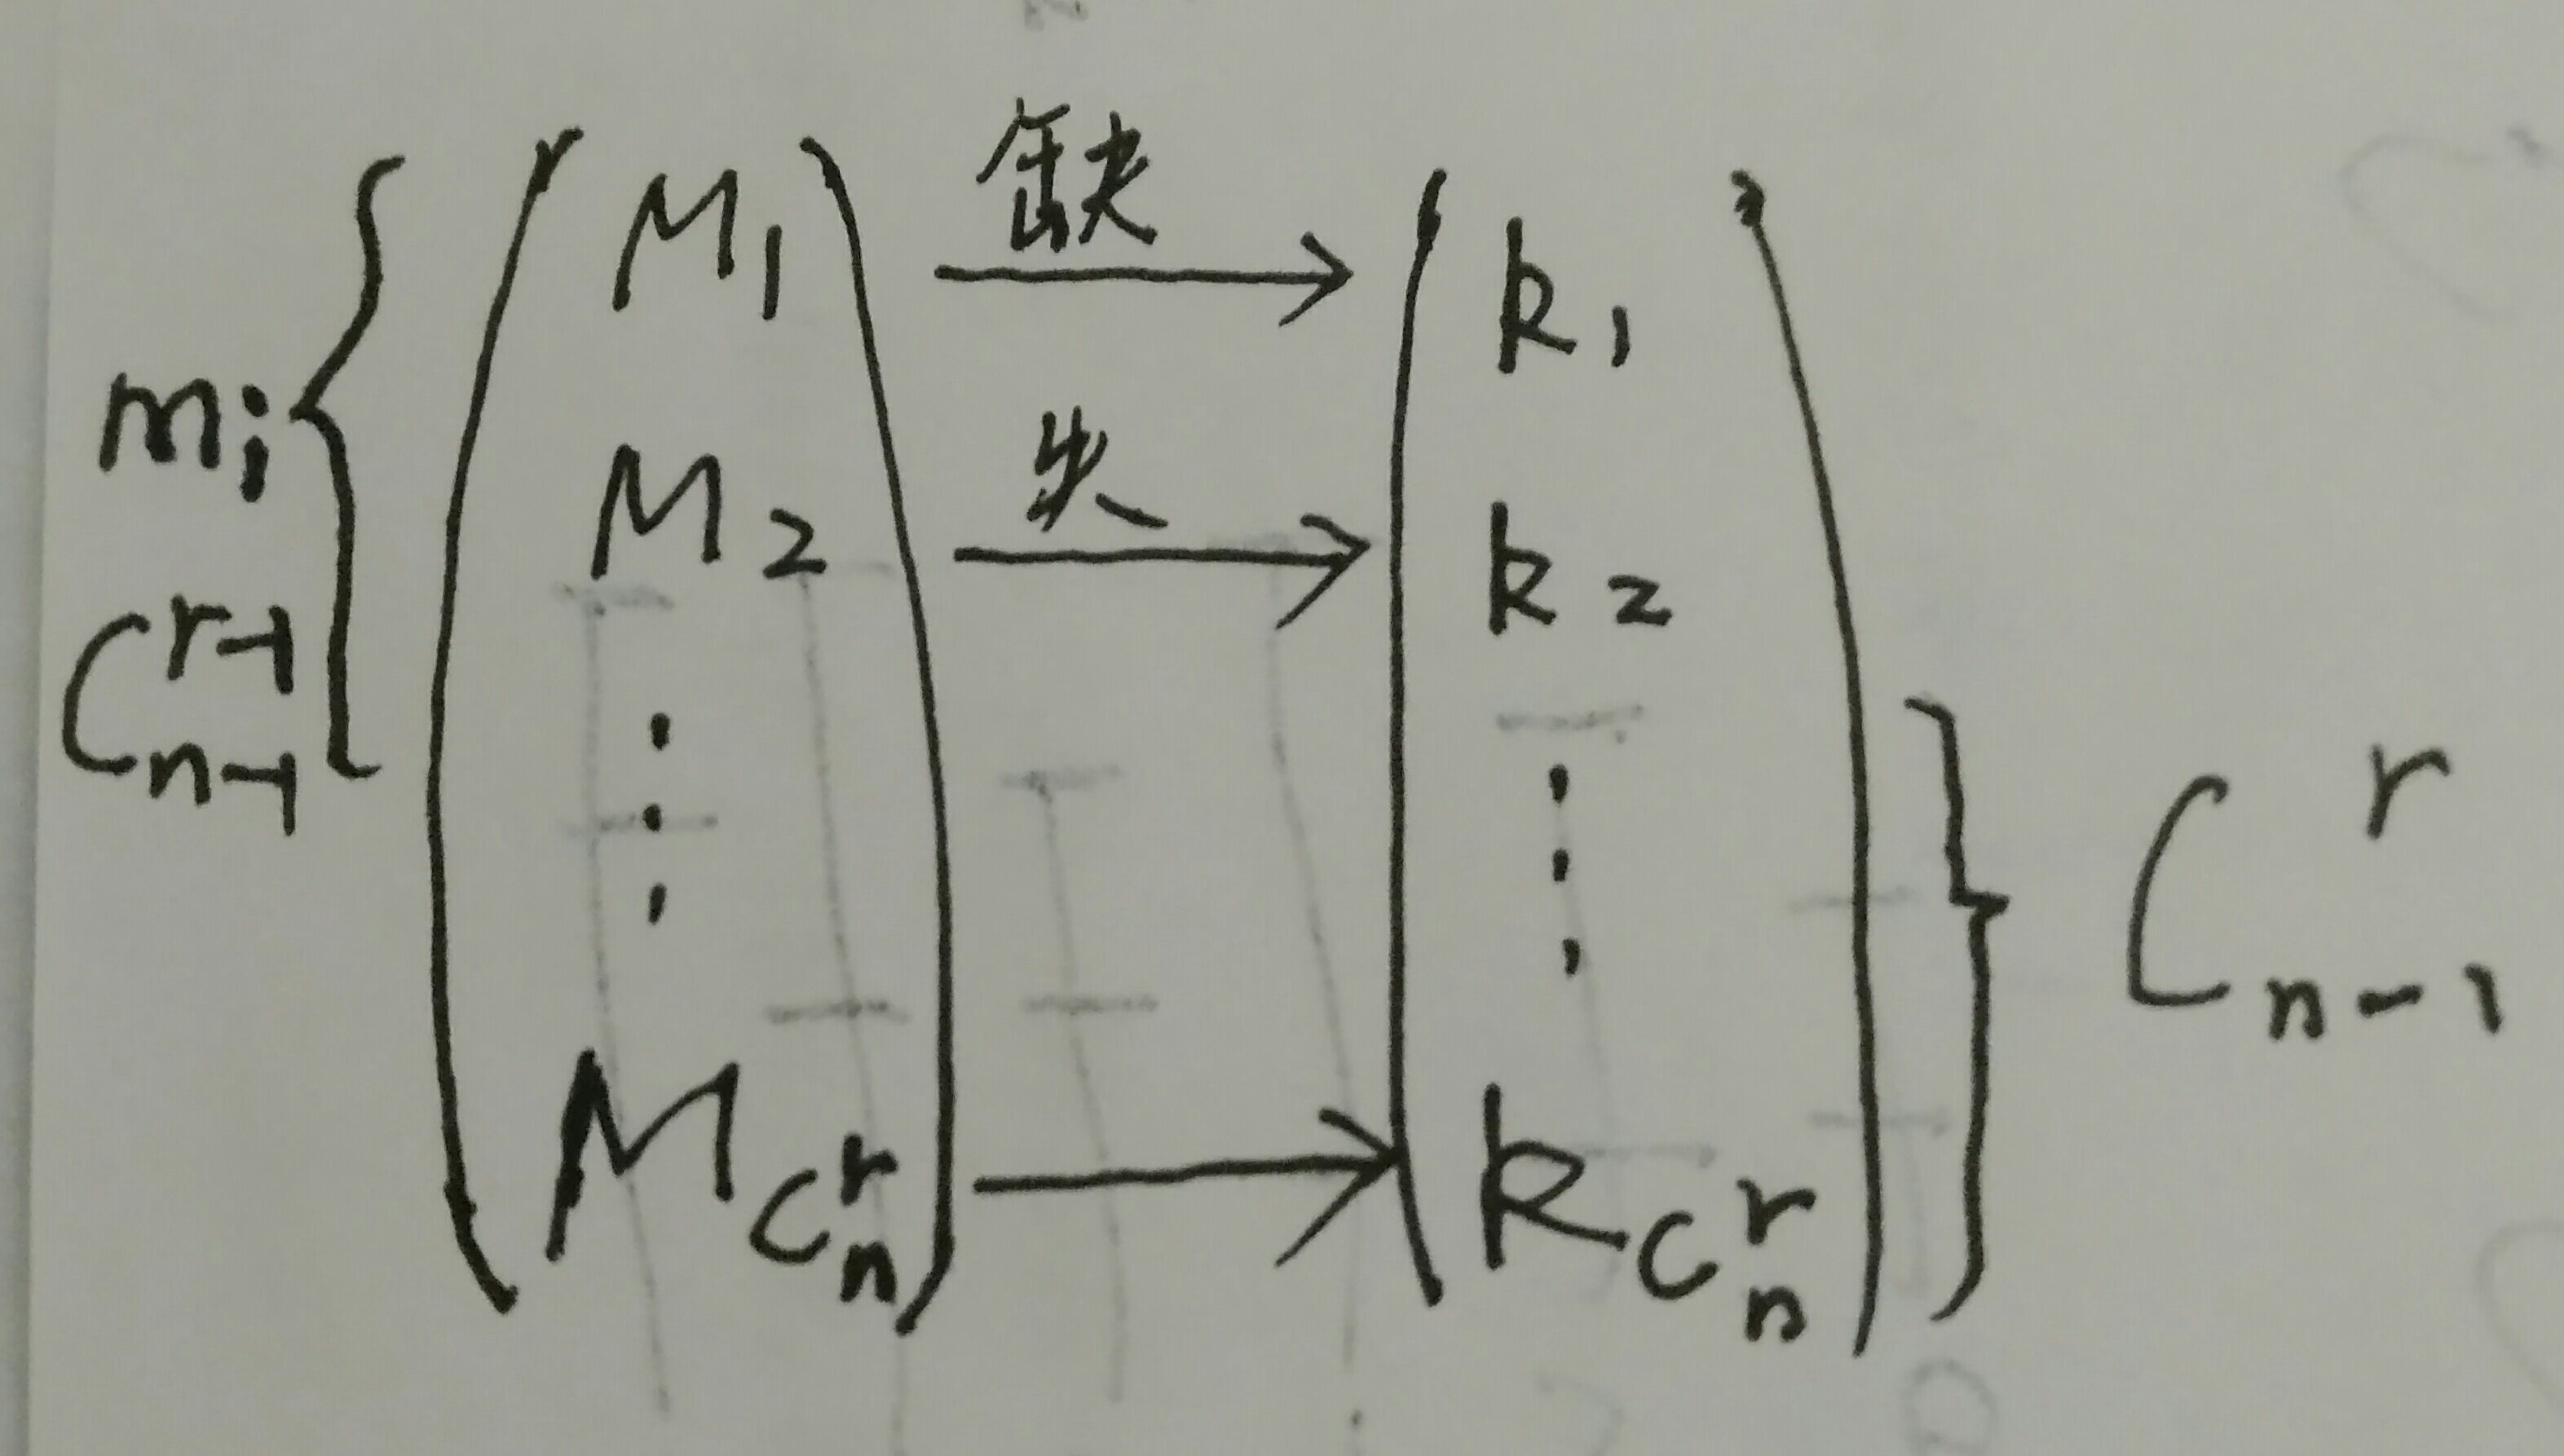
\includegraphics[width=.5\textwidth,scale=0.1]{injection}
\end{center}

对于某个管理员~$m_l$,~他所在~$r$~元素子集有~$C_{n - 1}^{r - 1}$~个,
到此,杨辉三角形公式里三个分项全部出现。很显然这管理员也缺失了这
些~$r$~元素子集对应的钥匙像,所以该管理员应分得剩下的~$C_{n -
  1}^r$~个钥匙像。针对所有管理员进行类似分配即可。

前面提过,当~$s,\, t$~的不等式不取等号时,此映射不是满射,有钥匙没有原
像,此时要求所有的~$r$~-组合都包含这样的钥匙。

现假设~$s = C_n^r + 1$,~此时的分配方案只需在原基础上稍加修改即可:
多出的这枚新钥匙再分配给每个管理员。这样~$t = C_{n - 1}^r + 1$.~此
设计仍满足保密要求。我们会发现这样的额外钥匙是没有必要的。每个管理
员都多了 1 枚同样的钥匙,起不到额外的安全作用。

分配方案的关键是根据~$s$~值列出~$r$元素子集到钥匙的
映射。现给出一个实际的例子。如果
~$n = 5,\, r = 3$,~则~$s = C_5^3 = 10,\, t = C_4^3 = 4$.~
下面给出一个映射。多出的一个钥匙(编号 11)是为了说明映射不一定是满射。

\begin{center}
  \begin{displaymath}
    \xymatrix@R=1mm{
      123 \ar[r]^{\text{缺}} & 1 \\
      124 \ar[r]            & 2 \\
      125 \ar[r]            & 3 \\
      134 \ar[r]            & 4 \\
      135 \ar[r]            & 5 \\
      145 \ar[r]            & 6 \\
      234 \ar[r]            & 7 \\
      235 \ar[r]            & 8 \\
      245 \ar[r]            & 9 \\
      345 \ar[r]            & 10 \\
                            & 11 }
  \end{displaymath}
\end{center}

每个管理员参与了~$C_{5 - 1}^{3 - 1} = 6$~个 3 元素子集,对应到映射
图上,有 6 行。不失一般性,管理员~$m_1$,~叁与了前 6 行,缺失前 6
枚钥匙,所以分得后 4 枚钥匙~$7,\, 8,\, 9,\, 10$.~依此类推,我们可
以得出如下分配方案。注意,该方案考虑到了第 11 枚钥匙。

\begin{table}[!htbp]
  \centering
  \begin{tabular}{c|*{11}c}
    \toprule
    \diagbox{Managers}{Keys} & 1 & 2 & 3 & 4 & 5 & 6 & 7 & 8 & 9 & 10 & 11 \\
    \midrule
    1 & 0 & 0 & 0 & 0 & 0 & 0 & 1 & 1 & 1 & 1 & 1 \\
    2 & 0 & 0 & 0 & 1 & 1 & 1 & 0 & 0 & 0 & 1 & 1 \\
    3 & 0 & 1 & 1 & 0 & 0 & 1 & 0 & 0 & 1 & 0 & 1 \\
    4 & 1 & 0 & 1 & 0 & 1 & 0 & 0 & 1 & 0 & 0 & 1 \\
    5 & 1 & 1 & 0 & 1 & 0 & 0 & 1 & 0 & 0 & 0 & 1 \\
    \bottomrule
  \end{tabular}
  \caption{Safe Device}
  \label{tab:safe-device}
\end{table}

\section{Permutation of Multiset}
\label{sec:permutation-multiset}

排列组合还会考虑所取元素元素是否\textbf{重复},从而生成(多)重排列
和(多)重组合。

前面两节介绍了单重集的排列组合,对应地,多重集也有排列组合,定义和
单重集一样,唯一的区别是取出的元素可能有重复。

设多重集~$M$~为:
\[ M = \{\; n_1 \cdot a_1,\; n_2 \cdot a_2,\; \dots,\;
  n_k \cdot a_k\; \},\quad \forall i = 1,\, 2,\, \cdots,\, k,\; r
  \leq n_i \]
或:
\[ M = \{\; \infty \cdot a_i,\; \infty \cdot a_2,\; \dots,\;
  \infty \cdot a_k\; \} \]
由于每种元素的个数超过所取数,所以排列里~$r$~个元素可能全部来自某
一种。

多重集~$M$~的~$r$-排列数是:\[ k^r \] 这是很容易理解的,因为队中每
个位置都有~$k$~种可能。

多重集~$r$-排列对应的彩球模型可以看成\textbf{可放回}(可重复)地对
单重集取球、排队或入盒。单重集里每个元素可无限重复使用,标记好队列
位置后又放回球堆里。当然按照多重集的定义,可以看成是对多重集取球、
排队或入盒。如不多于四位的三进制数的个数为~$3^4$.  ~对应的多重集
是
~$M = \{\, \infty \cdot 0,\, \infty \cdot 1,\, \infty \cdot 2\,
\}$.

如果~$r = n = \sum_{i = 1}^kn_i$,~则称为~$M$~的全排列。多重集全排
列(也即~$n$-排列)是对\textbf{有限集}~$M$~的\textbf{所有}元素
(如彩球)进行操作。具体来说,就是对全部~$n$个~$k$~种颜色的球进行排队。

显然此时~$r$~大于所有的~$n_i$. $M$~的全排列数为:
\[ \frac{n!}{ n_1!\, n_2!\, \cdots\, n_k! } \]

全排列的证明可以先从直觉来分析。~$n!$~表示所有元素的全排列,但
是~$a_i$~在队列重复了~$n_i$~次,这此重复实际只表示一种队列,所以除
以~$n_i!$.~如果某个~$n_i$~等于 1,~那么在被除式中是~1!.

有趣的是,实际证明中,用的是组合思路。第 1 种元素~$a_1$~要占据队列里
的~$n_1$~个位置,所以有~$C_n^{n_1}$~种可能,第二种元素要占据剩
下~$n - n_1$~个位置中的~$n_2$~个,所以有~$C_{n - n_1}^{n_2}$~种可
能,……,依此类推,最后一种元素有~$C_{n_k}^{n_k} = 1$~种可能:
\[ C_n^{n_1}\, C_{n - n_1}^{n_2}\, \cdots\, C_{n_k}^{n_k} = \frac{n!}{ n_1!\, n_2!\, \cdots\, n_k! } \]

从证明过程可知,当~$k = 2$~时,多得集的全排列数在数值上等于单重集的
组合数~$C_n^{n_1} = C_n^{n_2} = n!/(n_1!\, n_2!)$.~如用两面红旗,三
面黄旗依次悬挂在一根旗杆上,问可以组成多少种不同的标志?答案
是~$5!/(2!\, 3!) = 10$.

下面看一个棋盘的例子。在一个~$k \times k$~的棋盘上放~$k$~个车,使
得任意两个车之间不能互吃,有多少种方法?棋盘上车全是相同的,没有区
别。要想车不不互吃,任意两个车的行列值都不同。每行一个车
$a_{1\,j_1},\, a_{2\,j_2}\, \cdots\, a_{k\,j_k}$
,只需给不同行的车选列即可,所以方法数是~$k!$.

假设是~$k$~个不同(色)的车呢?保持上面排列不变,现对车的颜色进行
调换,有~$k!$~种,所以方法数是~$k! \, k!$.~实际是对车所在的行进行
全排列,也即行和列都要全排列。行的全排列负责车的不同,而列的全排列
负责车不互吃。

假设是~$n_1$~个红车,$n_2$~个蓝车,……,$n_k$~个黄车,总共~$n$~个呢?
先解决车在行上的全排列:$\frac{n!}{n_1!\, n_2!\, \cdots\, n_k!}$.
再针对不同的列全排列~$n!$.~方法数是:
\[ \frac{n!}{n_1!\, n_2!\, \cdots\, n_k!}\, \cdot\, n! \]

多重集~$r$-排列要求每种元素个数不少于~$r$,~若~$\exists t,\, n_t <
r$,~那么情问变复杂了。这时没有公式计算,要具体针对~$n_t$~列举分析。
如第~$t$~种元素出~$1,\, 2,\, \cdots,\, t$~个。

例:9 个元素的多重集~$S = {\, 3 \cdot a,\, 2 \cdot b, 4 \cdot c
  \,}$~的 8-排列数为多少?此例中,~$r = 8$~大于~$n_i$,~所以不能套
用公式。$n = 9$~只比~$r$~大 1,~所以列队中,~$a,\, b,\, c$~之一少出
一个元素。如少一个~$a$~排列数是~$\frac{8!}{2!\,2!\,4!}$,~同理可算
另两项,再用加法原则:
\[ \frac{8!}{2!\,2!\,4!} + \frac{8!}{3!\,1!\,4!} +
  \frac{8!}{3!\,2!\,3!} \]

\begin{figure}[!htbp]
  \centering
  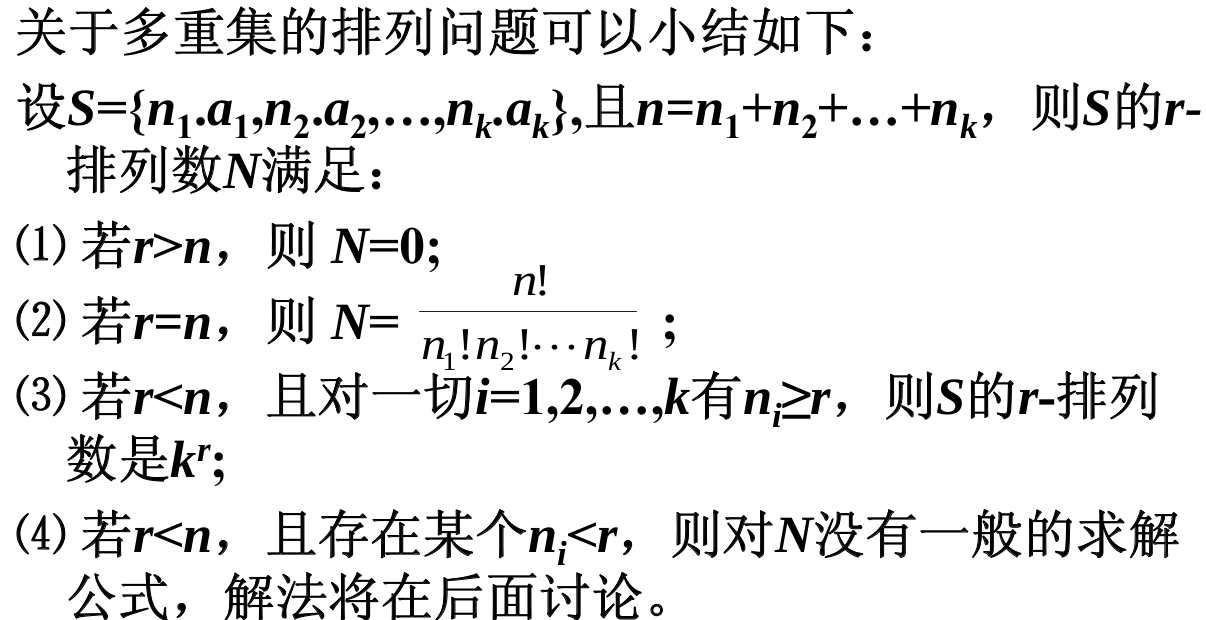
\includegraphics[width=1.0\textwidth]{SummPermMul}
  \caption{Summary on Multiset Permutation}
\end{figure}

\section{Combination of Multiset}
\label{sec:combination-multiset}

多重集~$S$~的含有~$r$~个元素的子多重集就叫做~$S$~的~$r$-组合,或表
述为取出~$r$~个元素的堆。和多重集的排列比少了列队操作。

同多重集的组合样,假设每种元素个数都不小于~$r$.~方法数即~$k$~元线
性不定方程:
\[ r = x_1\, +\, x_2\, +\, \cdots\, + x_k,\quad x_i \in
  \mathbb{Z}_0^+,\; i = 1,\, 2\, \cdots,\, k \] 的非负整数的解数。
\uwave{非负}是表明可能某~$x_t$~为 0, 此时元素~$a_t$~没有出现在组合
堆里。

计算用
\href{https://zh.wikipedia.org/zh-cn/\%E9\%9A\%94\%E6\%9D\%BF\%E6\%B3\%95}{
  隔板法}或
\href{https://zh.wikipedia.org/wiki/\%E6\%8F\%92\%E7\%A9\%BA\%E6\%B3\%95}{
  插空法}。

可以看成这样,有~$r$~个 1 在一行上,占有~$r$~位置,包含首尾共有~$r +
1$~个空位,插上~$k - 1$~个板子。第~$i$~板子前面的 1 个数是~$x_i$~的
解,第~$k - 1$~个板子后面的 1个数是~$x_k$~的解。如果某个板~$k_t$~前
没有 1 而是另一个板(两个板子处在同一空位),则~$x_t$~解为 0. 如从
\[ |\; 1\; |\; |\; 1\; 1\; \cdots\; 1\; 1\; | \] 
看出:
\[ x_1 = 0,\, x_2 = 1,\, x_3 = 0,\, x_k = 0 \]

非负正整数解的思路是:$r$~个 1 的位置和~$k - 1$~的板位置共~$r
+ (k - 1)$~个位置,从中取~$r$~个作为 1 的位置或取~$k - 1$~个作为板
的位置:
\[ C_{r + k - 1}^r \quad \text{or} \quad C_{r + k - 1}^{k - 1} \]

不考虑多重集组合,单就方程本身来说,如果是求正整数解呢?
\[ r = x_1\, +\, x_2\, +\, \cdots\, + x_k,\quad x_i \in
  \mathbb{Z}^+,\; i = 1,\, 2\, \cdots,\, k \]
正整数解暗含了~$r \geq k$,~非负解则无此限制。$r$~个 1 形中间有~$r
- 1$~个空档,插入~$k - 1$~个板,且每个空档最多一个板,则解数:
\[ C_{r - 1}^{k - 1} \]
这比非负情况的简单。

实际非负整数解和正整数解之间可以互相转换,形成一个满射,而解个数不
变。下面是把非负解转成正整数解的方法,即变量加 1:
\[ r\, +\, k =\, (x_1 + 1)\, +\, (x_2 + 1)\, +\, \cdots\, + (x_k + 1),\quad
  x_i \in \mathbb{Z}_0^+,\; i = 1,\, 2\, \cdots,\, k \]
新方程的解和原方程的解一一对应(满射:减一),这种变换思路很重要。
新方程的解是正整数解:
\[ C_{r + k - 1}^{k - 1} \]

把正整数解转成非负解,是把变量减 1.~利用转换原理,我们把方程:
\[ x_1 + x_2 + x_3 + x_4 = 20,\quad x_1 \geq 3,\, x_2 \geq 1,\,
  x_3 \geq 0,\, x_4 \geq 5 \]
转成非负解形式:
\[ (x_1 - 3) + (x_2 - 1) + (x_3 - 0) + (x_4 - 5) = 11,\quad x_1
  \geq 3,\, x_2 \geq 1,\, x_3 \geq 0,\, x_4 \geq 5 \]
或正整数解形式:
\[ (x_1 - 2) + (x_2 - 0) + [x_3 - (-1)] + (x_4 - 4) = 15,\quad x_1
  \geq 3,\, x_2 \geq 1,\, x_3 \geq 0,\, x_4 \geq 5 \]
后用插板法。

总结:

\begin{itemize}
\item 正整数:插板不相临;从中间空槽取~$k - 1$.
\item 非岁整数:插板可相监;从位数取~$k - 1$.
\end{itemize}

\section{Polynomial}
\label{sec:Polynomial}

这节谈下多项式和多重集排列、组合之间的联系。多项式:
\[ (x_1 + x_2 + \cdots + x_k)^n \]
的
\href{https://zh.wikipedia.org/zh-hans/\%E4\%BA\%8C\%E9\%A1\%B9\%E5\%BC\%8F\%E5\%AE\%9A\%E7\%90\%86#\%E5\%A4\%9A\%E9\%A1\%B9\%E5\%BC\%8F\%E5\%B1\%95\%E5\%BC\%80}{
  展开式}
可写成:
\[ \sum_{n_1 + n_2 + \cdots + n_k = n}\frac{n!}{n_1! n_2! \cdots
    n_k!}  x_1^{n_1} x_2^{n_2} \cdots x_k^{n_k},\quad n_i \in
  \mathbb{Z}_0^+: n_i \in [0,n],\; i = 0,1,\cdots,k \]
由此可看出,多项式的每项的系数是一个多重集的全排列数
$\frac{n!}{n_1! n_2! \cdots n_k!}$.~还可算出展开式的项数是多重集组
合数$\binom{n + k - 1}{n}$.

如果原多项式里~$x_i$~前还带有系数如~$a_i$:
\[ (a_1x_1 + a_2x_2 + \cdots + a_kx_k)^n \]
则情展开式的系数在多重集全排列数基础上还有乘以对应的原始系数。

如果问多项式的系数之和是多少,只需给所有~$x_i$~赋值 1 即可:
\[ (a_1 + a_2 + \cdots + a_k)^n \]
对于所有~$a_i = 1$~的情况,则系数和是~$k^n$.

\section{Grouping and Distribution}
\label{sec:group-distr}

下面是先说分组和分配问题,方法数和多重集全排列数有关。

\subsection{Distribution as Injection}
\label{sec:distr-inject}

将~$n = n_1\, +\, n_2\, +\, \cdots\, +\, n_k$~个 \textbf{不同}的
球~$a_i$~(单重集)放到~$k$~个 \textbf{不同}的对应盒子~$b_i$~里(单
重集)。~$b_1$~放~$n_1$~个,~$b_2$~放~$n_2$~个,……,~$b_k$~放~$n_k$
个。如果~$k = n$,~它就变成单重集的全排列,此时~$n_i = 1$.~简单描
述:\uline{把~$n$~个不同色球分成~$k$~堆~$n_i$,~依次分配给不同
  盒子~$b_i$}.

此模型称为\textbf{单重集的定向分配}问题。分配强调是分给\textbf{不
  同}的盒子,而定向是说~$n_i$~映射到~$b_i$,~每个盒子所分得
的\textbf{数量固定},\uline{即每堆的球数已经限定}。入盒操作相当于组
球堆贴标签。

计算过程和多重集全排列的类似,选取~$n_1$~个~$C_n^{n_1}$,~再在剩下
球里取~$n_2$~个~$C_{n - n_1}^{n_2}$, ……

这个取堆顺序是~$n_1,\, n_2,\, \cdots,\, n_k$,~实际按~$i$~的任何一
种排列顺序来取都可以,只要所取之堆放入对应的盒子子即可。如第一次
取~$n_5$个,~相当于给盒子~$b_5$~取球,那么取出后就放入盒子~$b_5$.

计算如下:
\[ C_n^{n_1}\,C_{n - n_1}^{n_2}\,\cdots\,C_{n_k}^{n_k} = \frac{n!}{ n_1!\, n_2!\, \cdots\, n_k! } \]
此计算利用了\uwave{乘法原则}。

最后,多重集全排列计算过程是给每种色球找队列位置(共~$n$~个),而上
面的模型是给每个盒子(共~$k$~个)选色球。此模型里彩球集合和空盒集合
是单重集,但放球后,盒子集合是多重集。每个盒子代表一种元素,里面的
球数代表这种元素的个数。

\subsection{Grouping}
\label{sec:grouping}

定向分配把球堆分给不同但固定的盒子,如取球放入~$k$~个的相同的盒子里
(盒子没有编号),此模型称为 \textbf{单重集的分组}问题。

由于盒子相同,所以有没有入盒操作对结果不影响,所以入盒是一个空操作。
所以有的题里,只提到分组,没有入盒操作(如分派给谁)。单重集分组可
以看成把取出球堆也堆在一起,形成一个大堆,大堆内元素是小球
堆:\uwave{分组即分堆}。

不失一般性,假设按~$n_1,\, n_2,\, \cdots,\, n_k$~的顺序取堆,如果
就此打住,那就成了定向分配。到底区别哪?没有\textbf{去重}!

球堆的区别是球个数~$n_i$~值的大小(球已取完,不再考虑其不同),可
能\uwave{某些堆的球数相等},这些堆算作是相同的堆。

不失一般性,假设~$n_1 = n_2 = n_3$~这 3 个堆球数相等,它们之间先取
谁后取谁没有变化,同理~$n_7 = n_9$~这 2 个堆的先后也不改变分组操作(没
有特殊说明,后面都据此假设)。所以要除掉重复:
\[ \frac{C_n^{n_1}\, C_{n - n_1}^{n_2}\, \cdots\, C_{n_k}^{n_k} }{
    3! \, 2! } \]
对所有的相同数值做类似去重除法即可。做题时,尽量把相同的~$n_i$~写
在一起,好去识别重复。

我们有理由把
\[ \{ n_1, n_2, \cdots, n_k \} \]
看成多重集:这~$k$~个值分成~$l$~种,每种里有~$t_j,\; j = 1, 2,
\cdots, l$~个元素,有~$\sum_{j = 1}^lt_j = k$.~拿上面的例子来说:
\[ \{ 3 \cdot n_1,\; 1 \cdot n_4,\; 1 \cdot n_5,\; 1 \cdot n_6,\;
  2 \cdot n_7,\; \cdots,\; 1 \cdot n_k \} \]
所以去重就是除以多重集每种元素个数的阶乘
~$t_1! \, t_2! \, \cdots \, t_j!$,~所以标准表达是:
\[ \frac{C_n^{n_1}\, C_{n - n_1}^{n_2}\, \cdots\, C_{n_k}^{n_k}
  }{t_1! \, t_2! \, \cdots \, t_j! } \]

一个特例是,所有~$n_i$~全相等,表示是\uline{平均分组},所以:
\[ \frac{C_n^{n_1}\, C_{n - n_1}^{n_2}\, \cdots\, C_{n_k}^{n_k} }{
    k! } = \frac{ n! }{ k! \, [ (\frac{ n }{ k })! ]^k } \]

再回过头看定向分配,发现可以分解成分组、定向分配 2 步:
\[ \frac{C_n^{n_1}\, C_{n - n_1}^{n_2}\, \cdots\, C_{n_k}^{n_k} }{
    3! \, 2! } \cdot\, 3! \, 2! \]
先把不同球数的堆放入对应的盒子。后面乘以~$3!$~表示~$n_1 = n_2 =
n_3$~这 3 个堆和~$b_1, b_2, b_3$~间可任意分派。乘以~$2!$~也是同
样的道理。

一句话:\textbf{分配问题暗含了分组子问题}。

\subsection{Distribution without Injection}
\label{sec:distr-with-inject}

有定向就有不定向,不定向分配也把球堆分派给不同的盒子,但是没有固定
分配关系:球堆~$n_i$~和盒子~$b_j$~间没有固定映射关
系。\uline{把~$n$~个不同色球分成~$k$~堆~$n_i$,~分配给不同盒
  子~$b_j$}.~此模型称为 \textbf{单重集的不定向分配}问题。

始终记住,盒子的不同、盒子编号代表队列位置。不定向分配分解成分组、
不定向分派 2 步:
\[ \frac{C_n^{n_1}\, C_{n - n_1}^{n_2}\, \cdots\, C_{n_k}^{n_k} }{
    3! \, 2! } \cdot\, k! \]
由于分组里已考虑到重复问题,后面的排列就不再考虑~$3! \, 2!$~重复,
而应把~$n_1 = n_2 = n_3$~看作是不同的堆,否则就会多次去重。

不定向分配还可以看成在定向分配基础上对~$k$~个球堆(数值~$n_i$)进行
全排列操作,方法数是:
\[ C_n^{n_1}\, C_{n - n_1}^{n_2}\, \cdots\, C_{n_k}^{n_k}\, \cdot
  \text{球堆全排队数} \]

在前节分组问题说到,堆的球数~$n_i$~是个多重集,所以我们乘以多
重集的全排列数:
\[
  \begin{aligned}[t]
    C_n^{n_1}\, C_{n - n_1}^{n_2}\, \cdots\, C_{n_k}^{n_k}\, \cdot
    \frac{ k! }{ 3! \, 2!}
    &= \frac{C_n^{n_1}\, C_{n - n_1}^{n_2}\, \cdots\, C_{n_k}^{n_k} }{
      3! \, 2! } \cdot\, k! \\
    &= \frac{n!}{ 3!\, 2!\, \cdot\, n_1!\, n_2!\, \cdots\, n_k! }\, \cdot\, k!
  \end{aligned}
\]
公式的推导过程也说明了不同的解题思路。

计算过程总结:

\begin{minipage}{1.0\linewidth}
  \begin{enumerate}
  \item 球一旦取出,组合计数完毕,就不再考虑球的不同。
  \item 取出的球堆区别于堆内球的个数。
  \item 可能某些堆球数相等,这些球堆看作是相同的堆。其实是一个多重
    集。
  \end{enumerate}
\end{minipage}

\subsection{Distribution of Multiset}
\label{sec:distr-mult}

上面的问题里,单重集每个球不同,如果所有球全相同呢?若像单重集分组
分配样规定~$n_i$,~则堆数确定,分组问题固定,只有 1 种方法。定向分
配问题:~$n$~个相同的球分成~$k$~组~$n_i$~定向派给不同盒子~$b_i$,~
也只有 1 种方法。不定向分配数是多重集的全排列如~$\frac{ k! }{ 3!
  \, 2! }$.

所以一般不规定堆内球数,如把~$n$~个同色球放入~$k$~个不同的盒子
里,盒子不为空。其实这个问题可化成求~$k$~元线性不定方程的正整数解。
方法数是:
\[ C_{n - 1}^{k - 1}\]

此时小球可看作是只有 1 种元素的多重集~$M = \{\, n \cdot a_1\, \}$.
此模型可称为含 1 种元素的\textbf{多重集定向分配}问题。

如果盒子可以为空,则化成求方程的非负整数解。

含一种元素的\textbf{多重集分组和不定向分配}问题没有统一解法,因为分
组和不定向要考虑去重问题,但是去重的前担是要知道~$n_i$~数值。所以只
能一一列举出方程解,再考虑每种解的去重,无法直接写出计数公式。

\section{Summary}

分组分配总结:

\begin{minipage}{1.0\linewidth}
  \begin{enumerate}
  \item 单重集分组:固序取堆、去~$n_i$~重。
  \item 单重集定向分配:固序取堆。
  \item 单重集不定向分配:固序取堆、去~$n_i$~重、排列。
  \item 多重集定向分配:插板法、解方程。
  \item 多重集分组和不定向分配:没有公式,只可一一列举。
  \end{enumerate}
\end{minipage}

% http://res.tongyi.com/resources/old_article/student/5869.html 加

\chapter{卡特兰数}
\label{cha:catalan-number}

\section{卡特兰公式}

\href{https://zh.wikipedia.org/zh-hans/\%E5\%8D\%A1\%E5\%A1\%94\%E5\%85\%B0\%E6\%95\%B0}{
  卡特兰数 Catalan Number} 在许多算法计数问题中都有应用,如出栈计数,
二叉树形态计数等。卡特兰数也叫明安图数。因为最提出这数的是中国明代
数学家明安图。但因为近代以来,科学技术主要由西方科学家发起,所以很
多发现用西方人物命名。

明安图数其实是一个组合数:

\[
  \begin{aligned}
    C_n = \frac{C_{2n}^n}{n+1} = \frac{1}{n+1} \binom{2n}{n} = \frac{(2n)!}{n!(n+1)!}
  \end{aligned}
\]

卡特兰数 $C_n$ 表示对 n 个元素的某种顺序计数。注意这里符号 $C_n$ 不
是前面的 n 个元素的组合数里的 $C_n^r$.

卡特兰数可以写成另外一种形式:

\begin{align*}
  C_n &= \frac{C_{2n}^n}{n+1} \\
      &= \frac{1}{n+1} \frac{(2n)\,!}{n\,!\, n\,!} \\
      &= \frac{1}{n(n+1)} \frac{(2n)\,!}{(n - 1)\,!\, n\,!} =
        (\frac{1}{n} - \frac{1}{n+1}) \frac{(2n)\,!}{(n - 1)\,!\,
        n\,!} \\
      &= \frac{1}{n} \frac{(2n)\,!}{(n - 1)\,!\, n\,!} - \frac{1}{n
        + 1} \frac{(2n)\,!}{(n - 1)\,!\, n\,!} =
        \frac{(2n)\,!}{n\,!\, n\,!} - \frac{(2n)\,!}{(n - 1)\,!\,
        (n + 1)\,!} \\
      &= C_{2n}^n - C_{2n}^{n + 1}
\end{align*}

请注意此化简过程用到

\[
  \frac{1}{n\,(n+1)} = \frac{1}{n} - \frac{1}{n+1}
\]

在处理组合数间题时,$\frac{1}{n-1}, \frac{1}{n}, \frac{1}{n+1}$ 经常被
用到来化简。这种倒数可以和阶成结合,组成新的组合数。

上面说的是卡特兰数结果,卡特兰数的递推关系式是:

\begin{align*}
  C_n &= \frac{C_{2n}^n}{n+1} \\
  &= \sum_{k=1}^n C_{k - 1}\,C_{n - k} \\
  &= C_0C_{n-1} + C_1C_{n-2} + \cdots + C_{n-1}C_0 \\
  &= \sum_{k=0}^{n-1} C_kC_{n-1-k}
\end{align*}

如何由这个递推关系得到结果式,要用到产生式或叫母函数 Generating
Function:

\begin{align*}
  g(x) = C_0x^0 + C_1x^1 + \cdots + C_{n-1}x^{n-1} + C_nx^n + \cdots
\end{align*}

关于如何用母函数求系数,细节请参考组合学课件,这里给出计算过程。上
面公式里,我们发现每项是子规模的乘积,所以对母函数平方:

\begin{align*}
  g^2(x) &= (C_0x^0 + C_1x^1 + \cdots + C_nx^n + \cdots)(C_0x^0 + C_1x^1 +
           \cdots + C_nx^n + \cdots) \\
         &= C_0^2x^0 + (C_0C_1 + C_1C_0)x^1 + \cdots + (C_0C_n +
           C_1C_{n-1} + \cdots + C_nC_0)x^n + \cdots \\
         &= C_1x^0 + C_2x^1 + \cdots + C_{n+1}x^n + \cdots \\
\end{align*}

对上式乘以 $x$ 得:

\begin{align*}
    x \cdot g^2(x) &= C_1x^1 + C_2x^2 + \cdots + C_nx^n + C_{n+1}x^{n+1} + \cdots
\end{align*}

对上式加 $C_0x^0 = 1$ 得:

\begin{align*}
  1 + x \cdot g^2(x) &= C_0x^0 + C_1x^1 + C_2x^2 + \cdots + C_nx^n
                       + \cdots \\
                     &= g(x) \\
  x \cdot g^2(x) - g(x) + 1 &= 0
\end{align*}

解上式得:

\begin{align*}
  g(x) = \frac{1 \pm \sqrt[2]{1-4x}}{2x}
\end{align*}

通过变换,得出母函数通项关系,去除系数 $C_k$, 进而解出母函数关
于$x$ 的表达式。$g(x)$ 是最开始的系数是由 $C_k$ 定义的,通过转换后
计算出系数,就得到 $C_k$.

根据二项式的推广:

\begin{align*}
  (x + y)^\alpha &= \sum_{k=0}^\infty \binom{\alpha}{k} x^k
                   y^{\alpha - k},\; a \in \mathbb{R} \\
  \binom{\alpha}{k} &= \frac{\alpha (\alpha - 1)\cdots(\alpha - k
                      + 1)}{k!}
\end{align*}

由此得:

\begin{align*}
  \sqrt[2]{1-4x} &= [1 + (-4x)]^{\frac{1}{2}} \\
                 &= \sum_{k=0}^\infty \binom{1/2}{k} (-4x)^k \\
                 &= 1 + \sum_{k=1}^\infty \binom{1/2}{k} (-4x)^k \\
                 &= 1 + \sum_{k=1}^\infty \frac{\frac{1}{2}\frac{-1}{2}\frac{-3}{2}\cdots\frac{3-2k}{2}}{k!} (-1)^k 2^{2k} x^k \\
                 &= 1 - \sum_{k=1}^\infty \frac{1 \,3 \cdots (2k - 3)}{k!} 2^k x^k \\
                 &= 1 - \sum_{k=1}^\infty \frac{1 (2 \cdot 1) \, 3 (2 \cdot 2) \cdots (2k - 3)[2 \cdot (k-1)]}{k!(k-1)!} \, 2x^k \\
                 &= 1 - \sum_{k=1}^\infty \frac{1 \, 2 \, 3 \, 4 \, \cdots \, (2k - 3)(2k - 2)}{k!(k-1)!} \, 2x^k \\
                 &= 1 - \sum_{k=1}^\infty \frac{[2(k - 1)]!}{k!(k-1)!} \, 2x^k
\end{align*}

结合上式得:

\begin{align*}
  g(x) &= \frac{1 \pm \sqrt[2]{1-4x}}{2x} \\
  &= \frac{1 \pm [1 - \sum_{k=1}^\infty \frac{[2(k - 1)]!}{k!(k-1)!} \, 2x^k]}{2x}
\end{align*}

考虑到定义时,系数 $C_k$ 是正数,所以正负号里选负号:

\begin{align*}
  g(x) &= \frac{1 \pm \sqrt[2]{1-4x}}{2x} \\
       &= \frac{1 \pm [1 - \sum_{k=1}^\infty \frac{[2(k -
         1)]!}{k!(k-1)!} \, 2x^k]}{2x} \\
       &= \frac{1 - [1 - \sum_{k=1}^\infty \frac{[2(k - 1)]!}{k!(k-1)!}
         \, 2x^k]}{2x} \\
       &= \sum_{k=1}^\infty \frac{[2(k - 1)]!}{k!(k-1)!} \, x^{k-1} \\
       &= \sum_{k=0}^\infty \frac{(2k)!}{k!(k+1)!} \, x^k
\end{align*}

通过系数对比,得出 $C_k = \frac{(2k)!}{k!(k+1)!} = \frac{1}{k+1}\,C_{2k}^k$.

\section{卡特兰数应用}

卡特兰数的来自于应用问题,~\ref{cha:algo-stack} 通过元素进出栈顺序
数问题,来说明公式推导过程。

长度为 $2n$ 的 Dyck Word(n 个 x 和 n 个 y 组成字符串)数;n 对括
号匹配组成合法运算式数;n 个节点组成二叉树方案数;$2n+1$ 个节点的满
二叉树数都是 $C_n$. 特别此 n 个节点的二叉树,添加 $n+1$ 个叶子节点,
形成满二叉树,个数都是 $C_n$.

二叉树前序序列和中序序列的关系。给定某二叉树前序序列或后序序列,求
中序序列的可能数,结果也是卡特兰数。相当于以前序序列或后序序列入栈,
中序序列出栈。

有 $n \times n$ 的小方格组成的正方形,要求从一个对角走到别一对角,
只能横向或竖向行走,不能回头且不能穿过对角线,问有多少种单调路径?
如从左下角往右上角行走,单调路径表示每一步只能向右或向上,即向最终
方向走。如果不考虑对角线问题,则竖向应走 n 步,横向应走 n 步,
共 $2n$ 步,方法数是$C_{2n}^n$. 若考虑对角线限制,假假沿在对角线下
方走,则说明任何时刻,右向步数不少于向上步数。肯体参考上面提到的进
出栈分析。

这些不同问题可以互相转化。如进栈、出栈,Dyck Word 里的 x 和 y, 左、
右括号都互相对应。全部用数学描述是 $2n$ 个 $\pm 1$ 串。

注意卡特兰数 $C_n$ 里有 n 表示规模,但是实际问题里,n 可能表示的是
n 对元素,而不是 n 个元素。如括号匹配里,n 对括号有 n 个左括号和 n
个右括号。

%%% Local Variables:
%%% mode: latex
%%% TeX-master: "main"
%%% End:
